\documentclass[10pt,twocolumn]{article}
\usepackage[letterpaper,margin=0.72in,columnsep=0.27in]{geometry}
\usepackage{lmodern}
\usepackage[T1]{fontenc}
\usepackage[utf8]{inputenc}
\usepackage{microtype}
\usepackage{amsmath,amssymb}
\usepackage{booktabs,tabularx,multirow}
\usepackage{graphicx}
\usepackage[table]{xcolor}
\usepackage{caption,subcaption}
\usepackage{enumitem}
\usepackage{tikz}
\usetikzlibrary{arrows.meta,positioning,fit,calc,decorations.pathreplacing,backgrounds,shapes.misc}
\usepackage[colorlinks=true,linkcolor=black,citecolor=black,urlcolor=blue!55!black]{hyperref}
\usepackage{titlesec}

% Generated by delivery_risk.final_report — do not edit by hand.
\newcommand{\RunId}{20261017T173852Z-64ef33}
\newcommand{\NOrders}{99{,}441}
\newcommand{\NApproved}{99{,}281}
\newcommand{\NScorable}{98{,}647}
\newcommand{\NLabelled}{96{,}394}
\newcommand{\NLate}{6{,}532}
\newcommand{\LateRate}{6.8\%}
\newcommand{\NScorableCanceled}{467}
\newcommand{\NScorableOther}{1{,}786}
\newcommand{\NUniqueCustomers}{96{,}096}
\newcommand{\NItems}{112{,}650}
\newcommand{\NMultiItem}{9{,}803}
\newcommand{\NMultiPayment}{2{,}961}
\newcommand{\NMultiReview}{547}
\newcommand{\NMultiSeller}{1{,}278}
\newcommand{\TrueItemValue}{13.59}
\newcommand{\NaiveItemValue}{14.14}
\newcommand{\NaiveRows}{117{,}329}
\newcommand{\FanoutPct}{4.0\%}
\newcommand{\NCritical}{24}
\newcommand{\NWarningsFired}{12}
\newcommand{\NChecks}{45}
\newcommand{\TestStart}{May 1, 2018}
\newcommand{\TestEnd}{August 1, 2018}
\newcommand{\TestScorable}{19{,}368}
\newcommand{\TestLabelled}{19{,}055}
\newcommand{\TestLate}{718}
\newcommand{\TestPrev}{3.8\%}
\newcommand{\TestCoverage}{98.4\%}
\newcommand{\NWeeks}{14}
\newcommand{\NBoot}{500}
\newcommand{\SelModel}{logistic regression}
\newcommand{\SelC}{0.1}
\newcommand{\SelCW}{balanced}
\newcommand{\SelAPLR}{0.070}
\newcommand{\SelAPLGB}{0.055}
\newcommand{\SelAPRule}{0.031}
\newcommand{\SelAPConst}{0.027}
\newcommand{\APSel}{0.075}
\newcommand{\APRule}{0.043}
\newcommand{\APConst}{0.038}
\newcommand{\APLGB}{0.090}
\newcommand{\APSelLo}{0.047}
\newcommand{\APSelHi}{0.115}
\newcommand{\AUCSel}{0.708}
\newcommand{\AUCLGB}{0.700}
\newcommand{\PtenSel}{8.7\%}
\newcommand{\PtenRule}{5.1\%}
\newcommand{\PtenLGB}{10.4\%}
\newcommand{\LiftSel}{2.30}
\newcommand{\DiffAP}{+0.032}
\newcommand{\DiffAPLo}{+0.015}
\newcommand{\DiffAPHi}{+0.060}
\newcommand{\DiffPten}{+3.4}
\newcommand{\DiffPtenLo}{-0.6}
\newcommand{\DiffPtenHi}{+9.5}
\newcommand{\DiffAPLGB}{+0.049}
\newcommand{\DiffAPLGBLo}{+0.033}
\newcommand{\DiffAPLGBHi}{+0.065}
\newcommand{\BrierRaw}{0.2520}
\newcommand{\BrierCal}{0.0455}
\newcommand{\BrierConst}{0.0364}
\newcommand{\CalPrev}{11.1\%}
\newcommand{\CalN}{11{,}178}
\newcommand{\CalSlope}{0.81}
\newcommand{\CalIntercept}{-2.14}
\newcommand{\SelLateKnown}{274}
\newcommand{\SelLateTotal}{1{,}287}
\newcommand{\SelKnownN}{10{,}025}
\newcommand{\TrainFitN}{40{,}906}
\newcommand{\TrainFitPos}{1{,}762}
\newcommand{\RefitN}{53{,}351}
\newcommand{\RefitPos}{2{,}707}
\newcommand{\CensTrain}{2{,}439}
\newcommand{\CensSel}{3{,}500}
\newcommand{\CensCal}{2{,}529}
\newcommand{\APMay}{0.138}
\newcommand{\PrevMay}{6.5\%}
\newcommand{\APJun}{0.034}
\newcommand{\PrevJun}{1.2\%}
\newcommand{\APJul}{0.048}
\newcommand{\PrevJul}{3.2\%}
\newcommand{\AblLR}{0.075}
\newcommand{\AblLGB}{0.092}
\newcommand{\CapEff}{10.2\%}
\newcommand{\CapPrec}{8.2\%}
\newcommand{\CapPrecRule}{5.4\%}
\newcommand{\CapKnownRate}{3.8\%}
\newcommand{\CapCaptured}{22.0\%}
\newcommand{\CapCapturedRule}{14.5\%}
\newcommand{\CapNoOutcome}{2.2\%}
\newcommand{\CapLift}{2.17}
\newcommand{\CapSelected}{1{,}976}
\newcommand{\CapDays}{91}
\newcommand{\CapMedianDaily}{197}
\newcommand{\CapCapturedTwenty}{38.2\%}
\newcommand{\QOneBefore}{300}
\newcommand{\QOneAfter}{4.2}
\newcommand{\QOneWindow}{11.3}
\newcommand{\QOneIdxMs}{384}
\newcommand{\QTwoBefore}{18.0}
\newcommand{\QTwoAfter}{13.3}
\newcommand{\QThreeBefore}{10.5}
\newcommand{\QThreeAfter}{0.22}
\newcommand{\NPredictions}{133{,}636}
\newcommand{\NTargets}{99{,}991}
\newcommand{\NOutcomeEvents}{97{,}733}
\newcommand{\DashOverviewCold}{251}
\newcommand{\DashOverviewWarm}{32}
\newcommand{\DashReviewCold}{63}
\newcommand{\DashReviewWarm}{1.7}
\newcommand{\PGVersion}{PostgreSQL 17.11}
\newcommand{\SplitSha}{64ef33ebf2ae}
\newcommand{\FeatureSha}{2da7b6cb19f0}
\newcommand{\PrecFiveSel}{8.8\%}
\newcommand{\ReviewLate}{2.27}
\newcommand{\ReviewOnTime}{4.29}
\newcommand{\LowLate}{62\%}
\newcommand{\LowOnTime}{9\%}
\newcommand{\RateCentralWest}{6.5\%}
\newcommand{\RateNorth}{8.6\%}
\newcommand{\RateNortheast}{12.7\%}
\newcommand{\RateSouth}{5.9\%}
\newcommand{\RateSoutheast}{6.1\%}
\newcommand{\PromiseShortRate}{21.5\%}
\newcommand{\PromiseShortN}{331}
\newcommand{\PromiseShortLo}{3}
\newcommand{\PromiseShortHi}{4}
\newcommand{\PromiseLongRate}{1.5\%}
\newcommand{\PromiseLongLo}{50}
\newcommand{\DistFirst}{4.3\%}
\newcommand{\DistLast}{11.7\%}
\newcommand{\DistLastLo}{1{,}457}
\newcommand{\LateNov}{12.2\%}
\newcommand{\LateFeb}{13.6\%}
\newcommand{\LateMar}{19.2\%}
\newcommand{\LateJun}{1.2\%}
\newcommand{\WarnNoItems}{775}
\newcommand{\WarnNoApproval}{160}
\newcommand{\WarnCarrier}{1{,}359}
\newcommand{\WarnNoCategory}{610}
\newcommand{\WarnGap}{303}
\newcommand{\WarnNoCentroid}{165}
\newcommand{\WarnNoDistance}{490}
\newcommand{\NFeatures}{27}
\newcommand{\NCandidates}{14}
\newcommand{\MinCoverage}{95.1\%}
\newcommand{\MinCoverageMonth}{January 2017}
\newcommand{\RiskRatio}{3.2}
\newcommand{\NNotScorable}{794}
\newcommand{\NNoOutcome}{2{,}253}
\newcommand{\NChecksTransform}{36}
\newcommand{\NChecksFeatures}{9}
\newcommand{\NCritTransform}{18}
\newcommand{\NCritFeatures}{6}


\definecolor{cblue}{HTML}{2A78D6}
\definecolor{corange}{HTML}{EB6834}
\definecolor{caqua}{HTML}{1BAF7A}
\definecolor{cgray}{HTML}{8A8984}
\definecolor{cviolet}{HTML}{6250D6}
\definecolor{cyellow}{HTML}{EDA100}
\definecolor{cred}{HTML}{C23B3A}
\definecolor{ink}{HTML}{1A1A1A}

\captionsetup{font=small,labelfont=bf,margin=0pt}
\setlength{\abovecaptionskip}{4pt}
\setlength{\belowcaptionskip}{0pt}
\setlength{\textfloatsep}{10pt plus 2pt minus 2pt}
\setlength{\floatsep}{8pt plus 2pt minus 2pt}
\setlength{\dbltextfloatsep}{10pt plus 2pt minus 2pt}
\setlist{nosep,leftmargin=1.1em}
\titlespacing*{\section}{0pt}{9pt plus 2pt}{4pt}
\titlespacing*{\subsection}{0pt}{6pt plus 2pt}{2pt}
\renewcommand{\arraystretch}{1.08}
\raggedbottom
\setcounter{dbltopnumber}{2}
\renewcommand{\dbltopfraction}{0.88}
\renewcommand{\dblfloatpagefraction}{0.75}
\renewcommand{\topfraction}{0.88}
\renewcommand{\textfraction}{0.08}
\renewcommand{\floatpagefraction}{0.75}
\newcommand{\code}[1]{\texttt{\small #1}}
\makeatletter
\newcommand{\inputtable}[1]{\@@input #1 }
\makeatother

\tikzset{
  box/.style={draw=#1!75!black, fill=#1!9, rounded corners=2pt, align=center, font=\scriptsize,
              text width=2.55cm, minimum height=1.05cm, inner sep=2pt},
  box/.default=cblue,
  arr/.style={-{Stealth[length=4pt]}, thick, draw=ink!70},
  txn/.style={draw=#1, dashed, rounded corners=4pt, inner sep=5pt},
}

\begin{document}

\twocolumn[{
\begin{center}
{\LARGE\bfseries Who Will Be Late? Prioritising Delivery-Risk Review at Order Approval}\\[5pt]
{\large A Leakage-Safe PostgreSQL Pipeline, a Frozen Temporal Evaluation and a\\Review-Capacity Simulation on \NOrders{} Olist Marketplace Orders}\\[7pt]
{\itshape Code: \href{https://github.com/yassineerraji/E-commerce-Delivery-Risk-Operations-Analytics}{GitHub Repository} \textbar{} App: \href{https://delivery-risk.onrender.com}{Live Dash application}}\\[6pt]
Yassine Erraji\\
October 2026
\end{center}
\vspace{2pt}
\noindent\textbf{Abstract}\quad
This report documents an end-to-end analytics system built on the public Olist marketplace export
(\NOrders{} orders, 2016--2018) to answer one operational question: when an order is approved, which
orders are most likely to arrive after the date promised to the customer, and how should a team with a
fixed review capacity prioritise them? Every transformation, from typed staging with quarantine to
point-in-time features, is written in PostgreSQL and guarded by \NChecks{} assertions, \NCritical{} of
which block publication. On the real data, a naive join of items, payments and reviews silently inflates
item value by \FanoutPct{}; the published tables reconcile exactly. Seller histories only use deliveries
that had already happened before approval, and an independent Python re-implementation reproduces all
\NTargets{} order--seller rows. Models are compared under a frozen four-block temporal protocol in which
an outcome becomes usable only once the parcel is delivered. On a 13-week test block (\TestLabelled{}
delivered orders, \TestPrev{} late), the logistic regression chosen beforehand reaches an average
precision of \APSel{}, against \APRule{} for a seller-history rule (paired weekly-bootstrap difference
\DiffAP{}, 95\% interval \DiffAPLo{} to \DiffAPHi{}) and \APConst{} without skill. Reviewing 10\% of each
day's approvals would have put \CapPrec{} late orders in the queue instead of \CapKnownRate{}, capturing
\CapCaptured{} of them. The report is equally explicit about what did not work: calibration learned on a
disrupted period over-estimates risk later, model selection saw only \SelLateKnown{} of \SelLateTotal{}
late examples because slow parcels arrive after the cut-off, and a LightGBM not selected in advance did
better on test. Nothing here shows that reviewing an order prevents a delay; Section~\ref{sec:limits}
describes the randomised pilot that would.
\vspace{10pt}
}]

% =====================================================================================
\section{Introduction}

A marketplace shows a delivery date at checkout and then depends on many independent sellers and
carriers to keep it. When the promise is broken, customers notice: in this dataset, orders delivered
late receive a mean review score of \ReviewLate{} out of 5, against \ReviewOnTime{} for orders delivered
on time, and \LowLate{} of late orders get a score of 1 or 2 (\LowOnTime{} of on-time orders). An
operations team can intervene before the delivery, for instance by contacting a seller or adjusting a
promise, but only for a small share of the orders it receives every day.

The decision studied here is therefore a \emph{ranking under capacity}: at the moment an order is
approved, sort the day's orders by estimated risk of late delivery and look at the top $q\%$.
Two properties make this harder than a standard classification exercise.
\emph{The data is relational}: an order can contain several items from several sellers, several
payments and several reviews, so any careless join multiplies rows. \emph{The data is temporal}: the
outcome of an order is only known once it is delivered, and the source is a final export rather than a
versioned event log, so it is easy to let information from the future leak into a feature or into
model selection.

The contribution is less a model than an \emph{evaluation discipline} applied end to end:
\begin{itemize}
\item a PostgreSQL pipeline whose grains, keys and totals are asserted before anything is published
      (Section~\ref{sec:pipeline});
\item point-in-time seller histories computed on delivery events, verified by mutation tests and an
      independent re-implementation (Section~\ref{sec:features});
\item a frozen temporal protocol with label-availability cut-offs, two baselines and paired block
      bootstrap intervals (Sections~\ref{sec:protocol}--\ref{sec:results});
\item a daily review-capacity simulation that separates what a reviewer would have seen from what
      can be evaluated afterwards (Section~\ref{sec:capacity});
\item a measured SQL performance study and a read-only analytics application
      (Sections~\ref{sec:perf}--\ref{sec:app}).
\end{itemize}

% =====================================================================================
\section{Data and Conventions}\label{sec:data}

\begin{figure*}[t]
\centering
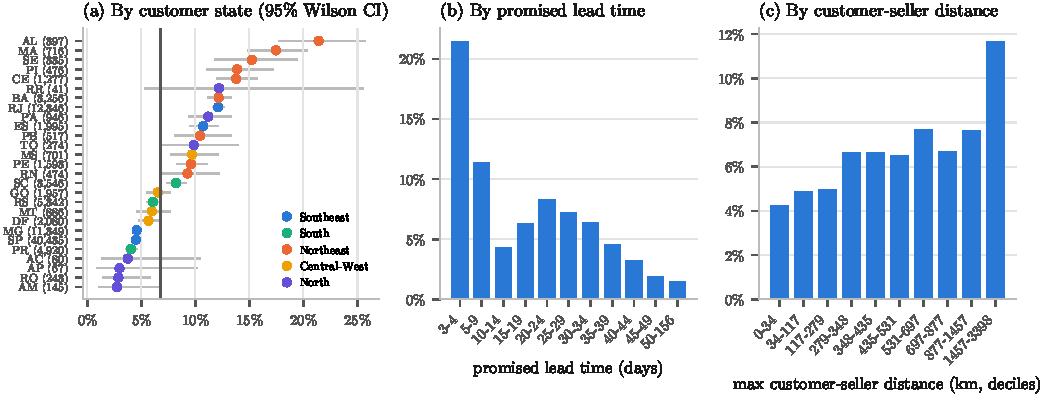
\includegraphics[width=\textwidth]{figures/diagnostic.pdf}
\caption{Late rate among eligible delivered orders. (a) Customer states with at least 30 orders,
95\% Wilson intervals, coloured by macro-region; the vertical line is the overall rate. (b) Promised
lead time (purchase to promised date). (c) Deciles of the largest customer--seller distance between
zip-prefix centroids.}
\label{fig:diagnostic}
\end{figure*}


The source is the \emph{Brazilian E-Commerce Public Dataset by Olist}, version 2 on Kaggle
(CC~BY-NC-SA~4.0)~\cite{olist}: nine CSV files describing orders placed between September 2016 and
October 2018. Each file is loaded as text with its batch, file name and physical line number, and a
manifest records its size, SHA-256 and record count (Table~\ref{tab:files}); re-importing an identical
file is a no-op.

\begin{table}[t]
\centering\small
\caption{Source files (current load). Records exclude headers; review messages span several physical
lines, which the loader reassembles.}
\label{tab:files}
\footnotesize
\begin{tabular}{@{}lrrl@{}}
\toprule
File & Records & MB & SHA-256 \\
\midrule
\inputtable{generated/table_files.tex}
\bottomrule
\end{tabular}
\end{table}

\paragraph{Conventions.} Prediction time is the approval timestamp; an order without approval is not
scored, and its purchase time is never used as a substitute. An order is \emph{late} when its delivered
\emph{date} is after its promised date. Dates rather than timestamps are compared because promises are
stored at midnight: a parcel delivered at 15:00 on the promised day is on time. Timestamps carry no
time zone in the source and none is invented. Item value, freight and payments are three distinct
measures, none of which is Olist's revenue or margin.

\paragraph{Populations.} Canceled, unavailable and undelivered orders are not ``on time''; they form
separate populations (Figure~\ref{fig:funnel}). An order is \emph{scorable} if the information
available at approval is coherent (approval present, promise not before purchase or approval, at least
one item). It is \emph{labelled} if, in addition, a delivery was observed after the approval. Every
exclusion carries a reason and appears in a coverage table.

\begin{figure}[t]
\centering
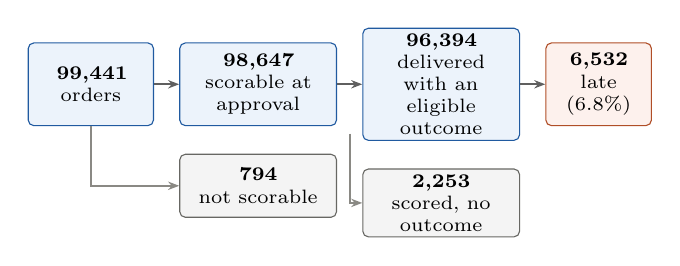
\begin{tikzpicture}[node distance=0.35cm and 0.32cm, font=\scriptsize]
\node[box=cblue, text width=1.45cm] (all) {\textbf{\NOrders}\\orders};
\node[box=cblue, text width=1.85cm, right=of all] (sc) {\textbf{\NScorable}\\scorable at\\approval};
\node[box=cblue, text width=1.85cm, right=of sc] (lab) {\textbf{\NLabelled}\\delivered with an\\eligible outcome};
\node[box=corange, text width=1.2cm, right=of lab] (late) {\textbf{\NLate}\\late\\(\LateRate)};
\node[box=cgray, text width=1.85cm, minimum height=0.8cm, below=of sc] (ns) {\textbf{\NNotScorable}\\not scorable};
\node[box=cgray, text width=1.85cm, minimum height=0.8cm, below=of lab] (no) {\textbf{\NNoOutcome}\\scored, no outcome};
\draw[arr] (all) -- (sc); \draw[arr] (sc) -- (lab); \draw[arr] (lab) -- (late);
\draw[arr, draw=cgray] (all.south) |- (ns.west);
\draw[arr, draw=cgray] ($(sc.south east)!0.5!(lab.south west)$) |- (no.west);
\end{tikzpicture}
\caption{Outcome populations. Not scorable: e.g.\ \WarnNoApproval{} orders without approval and orders
without items. Scored without outcome: \NScorableCanceled{} canceled or unavailable, the rest still in
transit at export. Features and scores exist for every scorable order; performance can only be measured
on the labelled ones.}
\label{fig:funnel}
\end{figure}

% =====================================================================================
\section{A Relational Pipeline in PostgreSQL}\label{sec:pipeline}

\begin{figure*}[t]
\centering
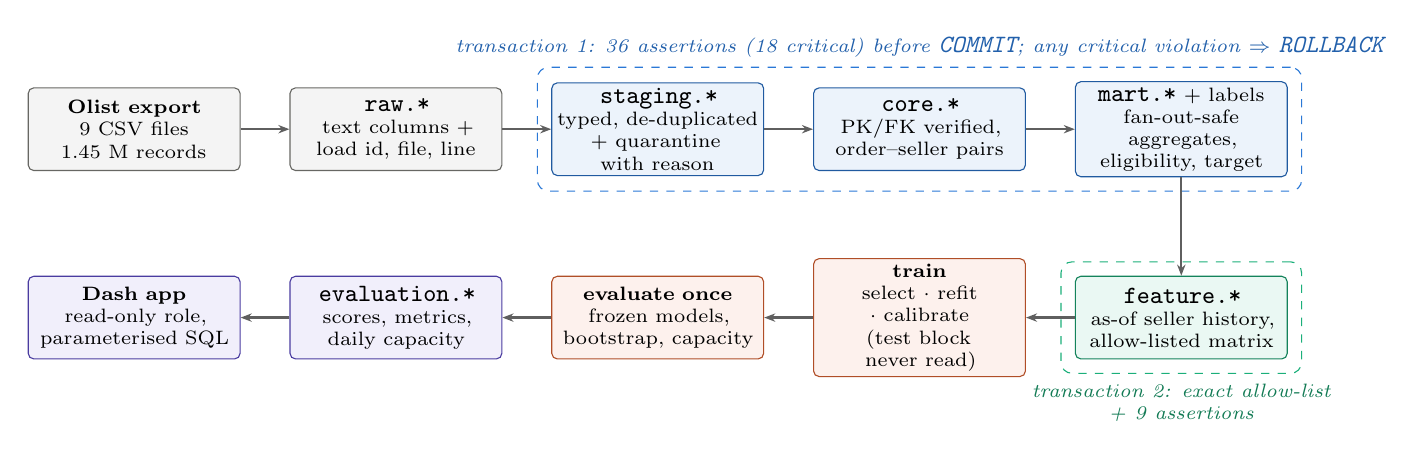
\begin{tikzpicture}[node distance=0.55cm and 0.62cm]
\node[box=cgray] (src) {\textbf{Olist export}\\9 CSV files\\1.45 M records};
\node[box=cgray, right=of src] (raw) {\code{raw.*}\\text columns +\\load id, file, line};
\node[box, right=of raw] (stg) {\code{staging.*}\\typed, de-duplicated\\+ quarantine with reason};
\node[box, right=of stg] (core) {\code{core.*}\\PK/FK verified,\\order--seller pairs};
\node[box, right=of core] (mart) {\code{mart.*} + labels\\fan-out-safe aggregates,\\eligibility, target};
\node[box=caqua, below=1.25cm of mart] (feat) {\code{feature.*}\\as-of seller history,\\allow-listed matrix};
\node[box=corange, left=of feat] (train) {\textbf{train}\\select $\cdot$ refit $\cdot$ calibrate\\(test block never read)};
\node[box=corange, left=of train] (eval) {\textbf{evaluate once}\\frozen models,\\bootstrap, capacity};
\node[box=cviolet, left=of eval] (evt) {\code{evaluation.*}\\scores, metrics,\\daily capacity};
\node[box=cviolet, left=of evt] (app) {\textbf{Dash app}\\read-only role,\\parameterised SQL};
\draw[arr] (src) -- (raw); \draw[arr] (raw) -- (stg); \draw[arr] (stg) -- (core); \draw[arr] (core) -- (mart);
\draw[arr] (mart) -- (feat); \draw[arr] (feat) -- (train); \draw[arr] (train) -- (eval); \draw[arr] (eval) -- (evt); \draw[arr] (evt) -- (app);
\begin{scope}[on background layer]
\node[txn=cblue, fit=(stg)(core)(mart), label={[font=\scriptsize\itshape, text=cblue!80!black, anchor=south]north:transaction 1: \NChecksTransform{} assertions (\NCritTransform{} critical) before \code{COMMIT}; any critical violation $\Rightarrow$ \code{ROLLBACK}}] {};
\node[txn=caqua, fit=(feat), label={[font=\scriptsize\itshape, text=caqua!70!black, align=center, anchor=north]south:transaction 2: exact allow-list\\+ \NChecksFeatures{} assertions}] {};
\end{scope}
\end{tikzpicture}
\caption{Pipeline. Each layer is rebuilt inside one transaction; because PostgreSQL DDL is
transactional, readers keep seeing the previous tables until the assertions pass. The dashboard reads
only \code{mart}, \code{evaluation}, \code{feature}, \code{quality} and \code{meta} with a read-only role.}
\label{fig:pipeline}
\end{figure*}

Figure~\ref{fig:pipeline} summarises the layers. \emph{Staging} casts every field with ordered
\code{CASE} checks (a cast only runs after its format check passed, which an \code{OR} would not
guarantee) and \code{pg\_input\_is\_valid}, so a malformed date is quarantined with a reason instead of
aborting the load. Rows sharing a key are split into strict duplicates (kept once and logged) and key
conflicts (all versions quarantined, publication blocked). \emph{Core} then adds primary and foreign
keys only after these checks. A child row whose parent was quarantined is cascaded with a warning, and
one whose parent does not exist at all is a critical orphan.

On the real files no row failed typing, no key conflicted and no reference was orphaned. All
\NCritTransform{} critical transform checks passed, and the anomalies that do exist are counted rather
than hidden: \WarnNoItems{} orders without items, \WarnNoApproval{} without approval, \WarnCarrier{}
carrier hand-offs recorded before approval, \WarnNoCategory{} products without category and \WarnGap{}
orders whose payments differ from items plus freight.

\paragraph{The fan-out trap.} Items, payments and reviews each hang under the order with their own
grain (\NMultiItem{} orders have several items, \NMultiPayment{} several payments, \NMultiReview{}
several reviews). Joining them directly on \code{order\_id} multiplies rows (Figure~\ref{fig:fanout}).
On the real data the naive join returns \NaiveRows{} rows instead of \NItems{} items and reports
R\$\NaiveItemValue{}\,M of item value instead of R\$\TrueItemValue{}\,M: a \FanoutPct{} error,
small enough to go unnoticed in a dashboard. The marts aggregate each child to the order grain first
and join one-to-one; an assertion compares every total before and after the join.

\begin{figure}[t]
\centering
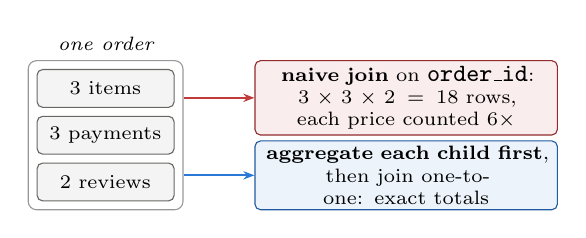
\begin{tikzpicture}[font=\scriptsize, node distance=0.1cm]
\node[box=cgray, text width=1.6cm, minimum height=0.48cm] (it) {3 items};
\node[box=cgray, text width=1.6cm, minimum height=0.48cm, below=of it] (pa) {3 payments};
\node[box=cgray, text width=1.6cm, minimum height=0.48cm, below=of pa] (re) {2 reviews};
\node[draw=ink!45, rounded corners=3pt, fit=(it)(pa)(re), inner sep=3pt, label={[font=\scriptsize\itshape]above:one order}] (ord) {};
\node[box=cred, text width=3.7cm, minimum height=0.85cm, anchor=north west] (bad) at ($(ord.north east)+(0.9,0)$)
  {\textbf{naive join} on \code{order\_id}:\\$3\times3\times2=18$ rows, each price counted $6\times$};
\node[box=cblue, text width=3.7cm, minimum height=0.85cm, anchor=south west] (good) at ($(ord.south east)+(0.9,0)$)
  {\textbf{aggregate each child first},\\then join one-to-one: exact totals};
\draw[arr, draw=cred] (ord.east |- bad.west) -- (bad.west);
\draw[arr, draw=cblue] (ord.east |- good.west) -- (good.west);
\end{tikzpicture}
\caption{The fan-out trap on one test-fixture order (130.00 of items becomes 780.00). On the real data
the same mistake inflates item value by \FanoutPct{}.}
\label{fig:fanout}
\end{figure}

\paragraph{Multi-seller orders.} \NMultiSeller{} orders involve more than one seller, but the delivery
timestamp exists only at order level. A seller's \emph{late-order exposure} therefore counts each order
once per seller through a distinct order--seller table; it is not a measure of seller-caused delay, and
seller counts do not add up to the marketplace total.

% =====================================================================================
\section{What the Operational Data Shows}\label{sec:diagnostic}

Of the \NLabelled{} delivered orders with an eligible outcome, \NLate{} were late
(\LateRate{}). Lateness is concentrated in time and space (Figure~\ref{fig:diagnostic}). It peaks with
the November~2017 Black Friday volume (\LateNov{} by approval month) and in February--March~2018
(\LateFeb{} and \LateMar{}), then falls to \LateJun{} in June~2018. Customers in the Northeast are late
\RateNortheast{} of the time, against \RateSoutheast{} in the Southeast. The rate also rises with
customer--seller distance, from \DistFirst{} in the nearest decile to \DistLast{} beyond
\DistLastLo{}~km. Promise length works the other way: very short promises
(\PromiseShortLo--\PromiseShortHi{} days, $n=$\PromiseShortN{}) are broken \PromiseShortRate{} of the
time, whereas promises of \PromiseLongLo{} days or more almost never are (\PromiseLongRate{}).
These are associations computed on delivered orders. They describe where risk sits; they do not say
that distance or promise length \emph{causes} delays.


% =====================================================================================
\section{Point-in-Time Features}\label{sec:features}





The matrix contains \NFeatures{} allow-listed features in four groups (Table~\ref{tab:features}).
Nothing observed after approval enters it, the classic source of leakage~\cite{kaufman2012}: no delivery date, no carrier hand-off, no status, no review,
no payment (payments lack a reliable availability log) and no raw identifier. The allow-list is checked
three times: when the matrix is built (an exact column comparison rolls the build back), by a SQL
assertion on column names, and by unit tests.

\begin{table}[t]
\centering\small
\caption{Feature groups. ``Assumed'' means plausible at approval but unverifiable in a final snapshot.}
\label{tab:features}
\footnotesize
\begin{tabularx}{\columnwidth}{@{}l c >{\raggedright\arraybackslash}X l@{}}
\toprule
Group & \# & Examples & At approval \\
\midrule
Order & 11 & promised lead days, item value, freight ratio, approval delay, shipping limit & assumed \\
Geography & 4 & customer state, seller state, same-state flag, distance & assumed \\
Catalog & 4 & main category, weight, volume, \# categories & assumed \\
Seller history & 8 & known outcomes, 90-day late rate, recent volume, no-history flag & observed \\
\bottomrule
\end{tabularx}
\end{table}

\paragraph{The as-of rule.} For an order approved at $t$, a past order of the same seller contributes an
outcome only if it was \emph{delivered} strictly before $t$ (Figure~\ref{fig:asof}). An order bought
before $t$ but still in transit at $t$ contributes nothing, and a delivery at exactly $t$ is excluded.
The 90-day window is anchored on delivery events, and approval-volume counters use approvals in
$[t-30\,\mathrm{d}, t)$. A moving average of final labels ordered by purchase date would violate this
rule, because it uses outcomes that were not yet known. Per-seller histories are averaged with equal
weight over the order's \emph{distinct} sellers, so a seller listed on two items counts once.

\begin{figure}[!ht]
\centering
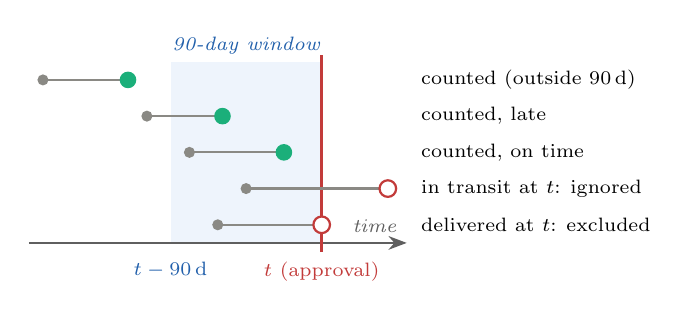
\begin{tikzpicture}[font=\scriptsize, x=0.6cm, y=0.46cm]
\fill[cblue!8] (3.0,-0.5) rectangle (6.2,4.5);
\node[font=\scriptsize\itshape, text=cblue!80!black] at (4.6,4.95) {90-day window};
\draw[-{Stealth}, thick, ink!70] (0,-0.5) -- (8.0,-0.5) node[above left, text=ink!70, font=\scriptsize\itshape] {time};
\draw[very thick, cred] (6.2,-0.75) -- (6.2,4.7);
\node[below, text=cred] at (6.2,-0.75) {$t$ (approval)};
\node[below, text=cblue!80!black] at (3.0,-0.75) {$t-90$\,d};
\foreach \y/\a/\d/\ok/\lab in {4/0.3/2.1/1/{counted (outside 90\,d)}, 3/2.5/4.1/1/{counted, late}, 2/3.4/5.4/1/{counted, on time},
                                 1/4.6/7.6/0/{in transit at $t$: ignored}, 0/4.0/6.2/0/{delivered at $t$: excluded}}{
  \draw[thick, cgray] (\a,\y) -- (\d,\y);
  \fill[cgray] (\a,\y) circle (2pt);
  \ifnum\ok=1 \fill[caqua] (\d,\y) circle (3pt); \else \draw[thick, cred, fill=white] (\d,\y) circle (3pt); \fi
  \node[anchor=west] at (8.1,\y) {\lab};
}
\end{tikzpicture}
\caption{Which past orders of a seller inform the score of an order approved at $t$. Each line runs
from a past order's approval (grey dot) to its delivery: green if strictly before $t$, red otherwise.}
\label{fig:asof}
\end{figure}

\begin{figure*}[t]
\centering
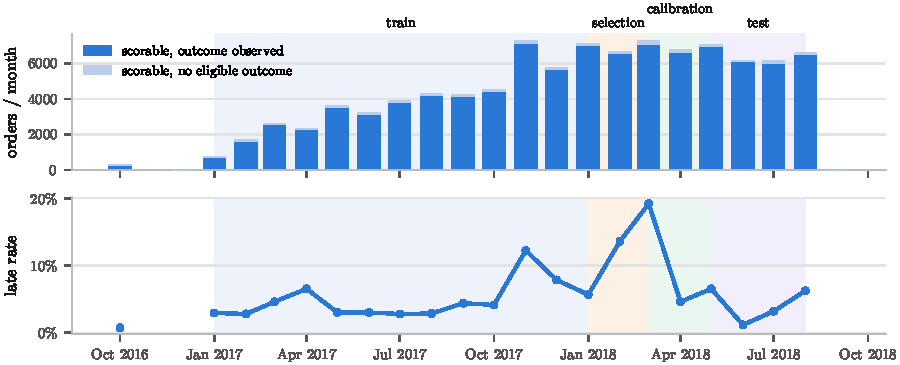
\includegraphics[width=\textwidth]{figures/timeline.pdf}
\caption{Scorable orders per approval month (light: no eligible outcome) and late rate, with the four
temporal blocks shaded. The calibration block falls in a disrupted period (late rate up to
\LateMar{}), whereas the test block is calm (\LateJun{} in June).}
\label{fig:timeline}

\vspace{14pt}
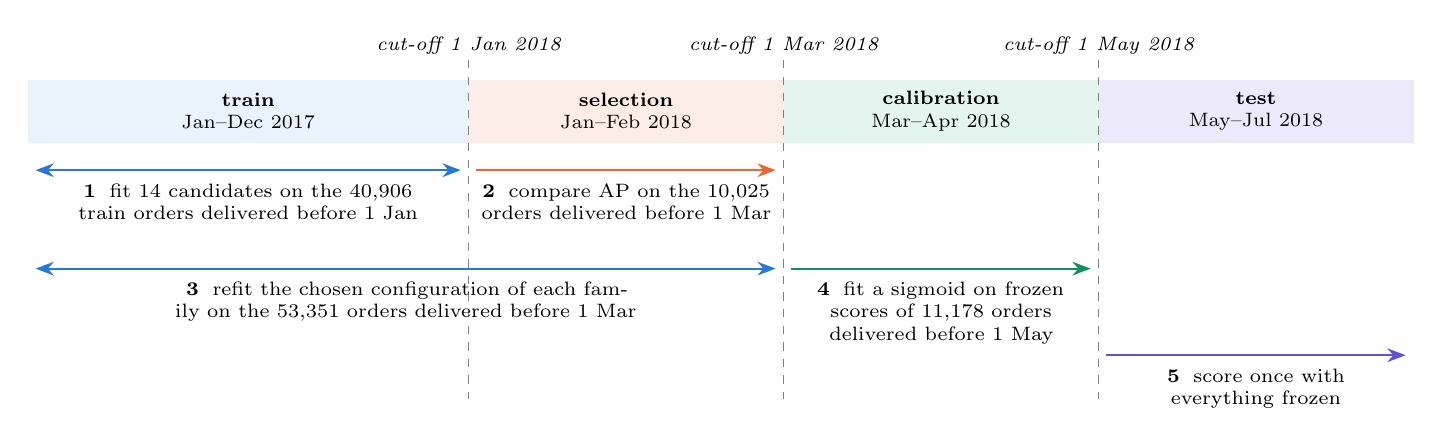
\begin{tikzpicture}[font=\scriptsize, x=1cm, y=1cm]
\fill[cblue!10] (0,0) rectangle (5.6,0.8);    \node[align=center] at (2.8,0.4) {\textbf{train}\\Jan--Dec 2017};
\fill[corange!12] (5.6,0) rectangle (9.6,0.8); \node[align=center] at (7.6,0.4) {\textbf{selection}\\Jan--Feb 2018};
\fill[caqua!12] (9.6,0) rectangle (13.6,0.8);  \node[align=center] at (11.6,0.4) {\textbf{calibration}\\Mar--Apr 2018};
\fill[cviolet!12] (13.6,0) rectangle (17.6,0.8); \node[align=center] at (15.6,0.4) {\textbf{test}\\May--Jul 2018};
\foreach \x/\d in {5.6/1 Jan 2018, 9.6/1 Mar 2018, 13.6/1 May 2018}{
  \draw[dashed, ink!55] (\x,1.05) -- (\x,-3.25);
  \node[above, font=\scriptsize\itshape] at (\x,1.0) {cut-off \d};
}
\draw[{Stealth}-{Stealth}, thick, cblue] (0.1,-0.35) -- (5.5,-0.35);
\node[below, text width=5.3cm, align=center] at (2.8,-0.4) {\textbf{1}\; fit \NCandidates{} candidates on the \TrainFitN{} train orders delivered before 1 Jan};
\draw[-{Stealth}, thick, corange] (5.7,-0.35) -- (9.5,-0.35);
\node[below, text width=3.8cm, align=center] at (7.6,-0.4) {\textbf{2}\; compare AP on the \SelKnownN{} orders delivered before 1 Mar};
\draw[{Stealth}-{Stealth}, thick, cblue] (0.1,-1.6) -- (9.5,-1.6);
\node[below, text width=9cm, align=center] at (4.8,-1.65) {\textbf{3}\; refit the chosen configuration of each family on the \RefitN{} orders delivered before 1 Mar};
\draw[-{Stealth}, thick, caqua!80!black] (9.7,-1.6) -- (13.5,-1.6);
\node[below, text width=3.8cm, align=center] at (11.6,-1.65) {\textbf{4}\; fit a sigmoid on frozen scores of \CalN{} orders delivered before 1 May};
\draw[-{Stealth}, thick, cviolet] (13.7,-2.7) -- (17.5,-2.7);
\node[below, text width=3.8cm, align=center] at (15.6,-2.75) {\textbf{5}\; score once with everything frozen};
\end{tikzpicture}
\caption{Training protocol (not to scale). At every step only labels whose delivery happened before the
next cut-off are used; models, preprocessing and calibrators are frozen before the test block is
scored.}
\label{fig:protocol}

\vspace{14pt}
\captionof{table}{Temporal blocks on the approval date ($[\text{start}, \text{end})$). The last two columns count
the labelled orders, and the late ones among them, that were already delivered at the next cut-off and
could therefore be used.}
\label{tab:blocks}
{\small
\begin{tabular}{@{}lllrrrrrr@{}}
\toprule
Block & Start & End & Scorable & Labelled & Late & Late rate & Usable at cut-off & Late usable \\
\midrule
\inputtable{generated/table_blocks.tex}
\bottomrule
\end{tabular}
}
\end{figure*}

\begin{figure*}[t]
\centering
\captionof{table}{Test block (\TestStart{} to \TestEnd{}, exclusive): \TestLabelled{} delivered orders with an
eligible outcome, \TestLate{} late (prevalence \TestPrev{}). $^\star$Selected on the selection block before
the test was scored. Brier scores before and after the sigmoid calibrator; ranking metrics are
unchanged by calibration.}
\label{tab:models}
{\footnotesize\setlength{\tabcolsep}{5pt}
\begin{tabular}{@{}lrcrrrrrr@{}}
\toprule
Model & AP & 95\% CI & ROC-AUC & Precision@10\% & Recall@10\% & Lift@10\% & Brier raw & Brier calibrated \\
\midrule
\inputtable{generated/table_models.tex}
\bottomrule
\end{tabular}
}
\vspace{16pt}
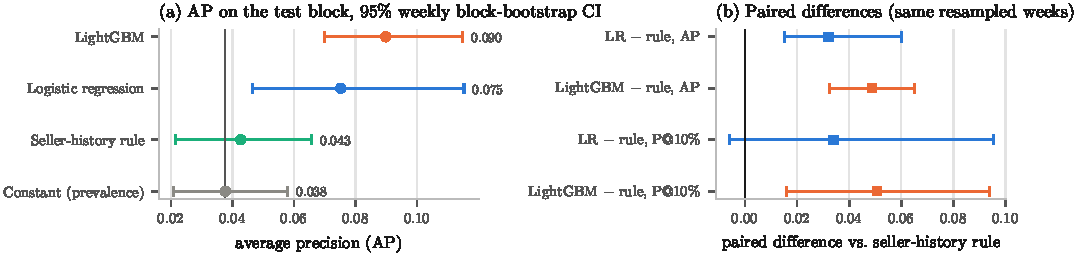
\includegraphics[width=\textwidth]{figures/ap_ci.pdf}
\captionof{figure}{(a) Average precision with 95\% weekly block-bootstrap intervals; the vertical line is the
no-skill value (prevalence). (b) Paired differences against the seller-history rule, computed on the
same resampled weeks.}
\label{fig:ap}
\end{figure*}


\paragraph{Verification.} Hand-written fixtures pin the expected values of each rule. One test moves a
delivery from exactly $t$ to one second earlier and checks that it then counts. Mutation tests rewrite
future deliveries and reviews, or add future orders, and assert that every feature of earlier orders is
byte-identical. Finally, an independent Python implementation was run against the SQL on the full real
dataset and agreed on all \NTargets{} order--seller rows.

A known bias remains: histories describe \emph{delivered} orders, so a seller whose parcels are
currently stuck looks better than it is until they arrive.

% =====================================================================================
\section{Temporal Evaluation Protocol}\label{sec:protocol}




Four contiguous calendar blocks are defined on the approval date (Figure~\ref{fig:timeline},
Table~\ref{tab:blocks}). Their boundaries were proposed from public coverage information and confirmed
unchanged by a coverage audit of the downloaded files, \emph{before any model was trained}. The audit
reports volumes, label coverage, label delays and late counts per month and per block; label coverage
is at least \MinCoverage{} in every month of the blocks (lowest in \MinCoverageMonth). The definition is hashed (\code{\SplitSha}) and training refuses
any block definition that is not frozen.





\begin{figure*}[t]
\centering
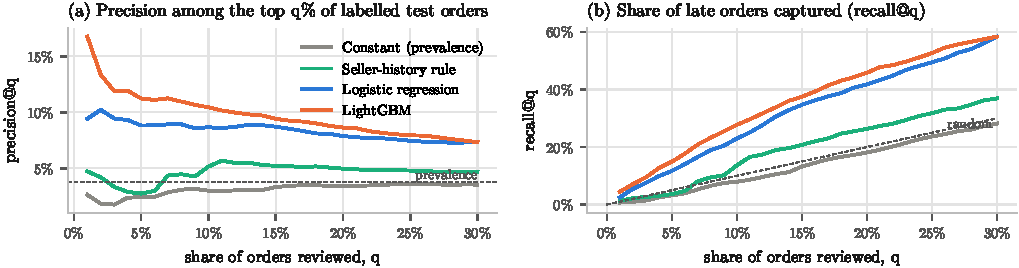
\includegraphics[width=\textwidth]{figures/topq.pdf}
\caption{Global top-$q$ curves on the labelled test orders. The dashed lines are the prevalence (a) and
random selection (b); vertical guides mark 5, 10 and 20\%.}
\label{fig:topq}
\end{figure*}

\paragraph{Label availability.} An outcome is usable from the actual customer delivery, including for
late orders. Figure~\ref{fig:protocol} shows the five steps. Candidates are fitted on train orders
delivered before the selection cut-off. A fixed grid (4 logistic regressions, 8 LightGBM~\cite{lightgbm}
configurations, written down before any result) is compared by average precision on selection orders
delivered before the calibration cut-off. The chosen configuration of each family is refitted on train
plus selection, and a sigmoid calibrator is fitted on the frozen scores of the calibration block. The
test block is then scored once.
The cut-offs have a cost, visible in Table~\ref{tab:blocks}: late parcels arrive after on-time ones, so
when the model was chosen only \SelLateKnown{} of the \SelLateTotal{} late selection orders had been
delivered. This is what a real deployment would have known at that date, and it makes model choice
noisy.

\paragraph{Metrics.} The headline metric is average precision (AP, scikit-learn's step-wise
definition~\cite{sklearn}), which focuses on the top of the ranking and whose no-skill value is the
prevalence; with \TestPrev{} positives, ROC-AUC would flatter weak rankings~\cite{saito2015}.
Precision, recall and lift at $q$ use $k=\lceil qN\rceil$ with ties broken by order id. Uncertainty
comes from a paired bootstrap that resamples whole ISO weeks of the test block (\NBoot{} resamples,
\NWeeks{} weeks)~\cite{kunsch1989}, so that every model is scored on the same resampled weeks. Every
evaluation is logged; re-running it on the same run is recorded as a verification, and a model trained
after a test evaluation would be flagged as exploration.

% =====================================================================================
\section{Results}\label{sec:results}

\begin{figure*}[t]
\centering
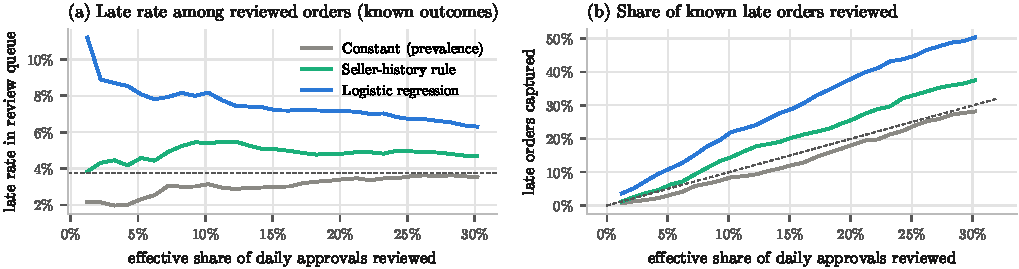
\includegraphics[width=\textwidth]{figures/capacity.pdf}
\caption{Daily review policy over the \CapDays{} test days. (a) Late rate among reviewed orders with a
known outcome; the dashed line is the late rate of all known orders. (b) Share of all known late orders
that were reviewed; the dashed diagonal is random selection.}
\label{fig:capacity}
\end{figure*}




\paragraph{The model beats the rule on AP, modestly.} The selected \SelModel{} ($C=\SelC$, class weight
\SelCW) reaches an AP of \APSel{} on the test block, against \APRule{} for the seller-history rule and
\APConst{} for a constant score (Table~\ref{tab:models}). The paired difference with the rule is
\DiffAP{} (95\% interval \DiffAPLo{} to \DiffAPHi{}) and is positive in every resample
(Figure~\ref{fig:ap}). At the 10\% operating point the picture is less clear-cut: precision rises from
\PtenRule{} to \PtenSel{}, a lift of \LiftSel{} over the prevalence, but the paired difference
(\DiffPten{} points, interval \DiffPtenLo{} to \DiffPtenHi) includes zero. The absolute level stays
modest: more than nine reviewed orders in ten would have arrived on time anyway.

\paragraph{The model selected in advance was not the best one.} LightGBM, which lost the selection
(selection AP \SelAPLGB{} vs \SelAPLR{}), does better on test: AP \APLGB{}, difference with the rule
\DiffAPLGB{} (\DiffAPLGBLo{} to \DiffAPLGBHi), and \PtenLGB{} precision at 10\%. It is not substituted
afterwards: choosing it now would turn the test block into a second selection set. The likely cause is
the noisy selection described above (\SelLateKnown{} late examples, drawn from a disrupted period).
This is a property of the evaluation design to keep, not an anomaly to correct.



\paragraph{Performance moves with the late rate.} Ranking quality is far from uniform over the test
weeks (Figure~\ref{fig:months}). In May~2018, with a \PrevMay{} late rate, the selected model's AP is
\APMay{}; in June, when only \PrevJun{} of orders were late, it falls to \APJun{} (July: \APJul{} at
\PrevJul{}). Rare-event months leave little signal to find, and 14 weeks give wide intervals. The
results should be read as an order of magnitude, not as a stable operating characteristic.

\begin{figure}[t]
\centering
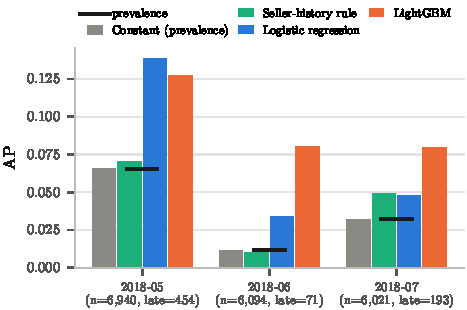
\includegraphics[width=\columnwidth]{figures/months.pdf}
\caption{AP by test month; black ticks mark the month's late rate (no-skill AP).}
\label{fig:months}
\end{figure}

\paragraph{Calibration does not transfer across seasons.} Class weighting makes the raw logistic scores
far too high (Brier \BrierRaw). The sigmoid calibrator~\cite{platt1999,niculescu2005} learned on the
calibration block (\CalN{} orders, \CalPrev{} late) brings the Brier score to \BrierCal{}, which is
still worse than the constant prevalence (\BrierConst). Because the calibration months were about
\RiskRatio{} times as risky as the test months, calibrated probabilities over-estimate risk (Figure~\ref{fig:calib}).
Rankings are unaffected, so the score can be used to \emph{order} orders. To read it as a probability,
it must first be recalibrated on recent deliveries.

\begin{figure}[t]
\centering
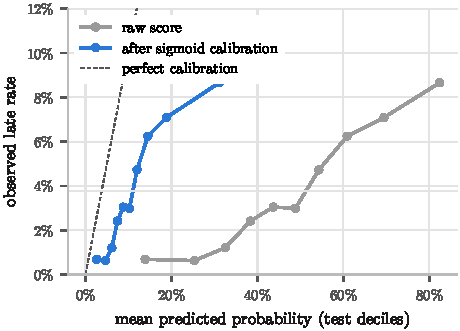
\includegraphics[width=\columnwidth]{figures/calibration.pdf}
\caption{Calibration of the selected model on test deciles. The calibrator learned an \CalPrev{} late
rate; the test rate is \TestPrev{} (horizontal line).}
\label{fig:calib}
\end{figure}

\paragraph{Sensitivity and interpretation.} The catalog attributes (category, weight, volume) come from
a final product snapshot and are only \emph{assumed} to be known at approval. Retraining without them
leaves AP unchanged (\AblLR{} for logistic regression, \AblLGB{} for LightGBM), so the results do not rest
on that assumption. Permutation importance on the calibration block (Figure~\ref{fig:imp}) ranks
seller-history support, customer state, promised lead time, same-state and distance features first.
Consistent with Section~\ref{sec:diagnostic}, these are associations within this dataset and do not
identify causes.

\begin{figure}[t]
\centering
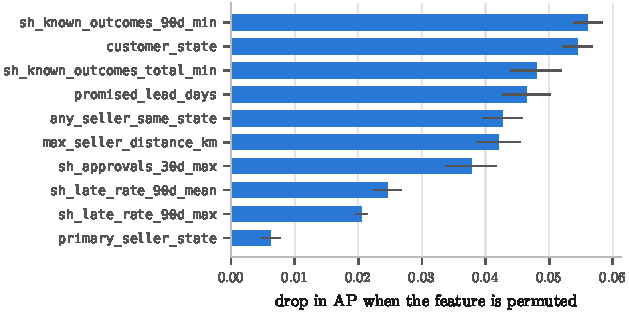
\includegraphics[width=\columnwidth]{figures/importance.pdf}
\caption{Permutation importance of the selected model (AP drop, 5 repeats) on the calibration block,
never on test.}
\label{fig:imp}
\end{figure}

% =====================================================================================
\section{From Scores to a Review Policy}\label{sec:capacity}

The global top-$q$ above ranks all labelled test orders at once, which is right for comparing models
but not how a team works. The operational simulation replays each historical day: all orders approved
that day are ranked by the score frozen at approval, and the top $\lceil qN_{\text{day}}\rceil$ are
\emph{selected before any outcome exists}. Only afterwards are outcomes looked up; some selected orders
never get one (canceled or undelivered), and this share is reported rather than dropped. The rounding
makes the reviewed share slightly larger than $q$ (\CapEff{} for $q=10\%$, with a median of
\CapMedianDaily{} approvals per day).


\begin{table}[t]
\centering\footnotesize
\setlength{\tabcolsep}{2.6pt}
\caption{Daily review policy. ``Known'' is the share of selected orders with an observable outcome;
``Late'' is computed among those; ``Captured'' is the share of all known late orders reviewed.}
\label{tab:capacity}
\begin{tabular}{@{}lrrrrrr@{}}
\toprule
Ranking & $q$ & Reviewed & Known & Late & Lift & Captured \\
\midrule
\inputtable{generated/table_capacity.tex}
\bottomrule
\end{tabular}
\end{table}

With a 10\% daily capacity, the selected model puts \CapPrec{} late orders in the review queue, against
\CapPrecRule{} for the seller-history rule and \CapKnownRate{} on average (a lift of \CapLift), and the
queue contains \CapCaptured{} of all known late orders (\CapCapturedRule{} for the rule). Doubling the
capacity to 20\% raises the share captured to \CapCapturedTwenty{} (Table~\ref{tab:capacity},
Figure~\ref{fig:capacity}). Only \CapNoOutcome{} of the selected orders have no observable outcome, so
the selection bias from undelivered orders is small on this window.

These figures describe \emph{targeting}. They do not show that reviewing an order changes its outcome,
and no saving or delay reduction is claimed.

% =====================================================================================
\section{SQL Performance}\label{sec:perf}

\begin{figure*}[p]
\centering
\begin{subfigure}{\textwidth}\centering
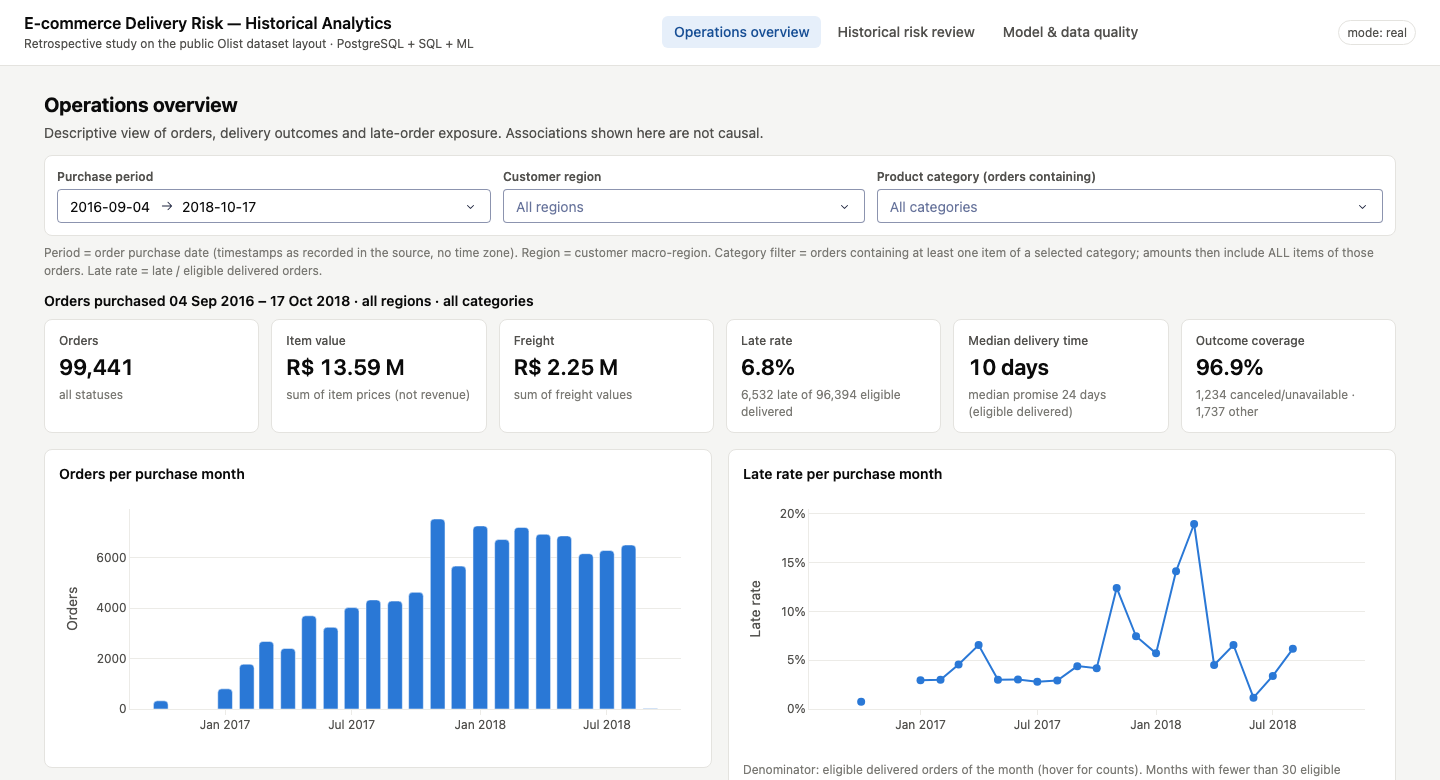
\includegraphics[width=0.9\linewidth]{figures/overview_1440_crop.png}
\caption{Operations overview, all filters off: KPIs with their denominators and monthly trends.}
\end{subfigure}\\[8pt]
\begin{subfigure}{\textwidth}\centering
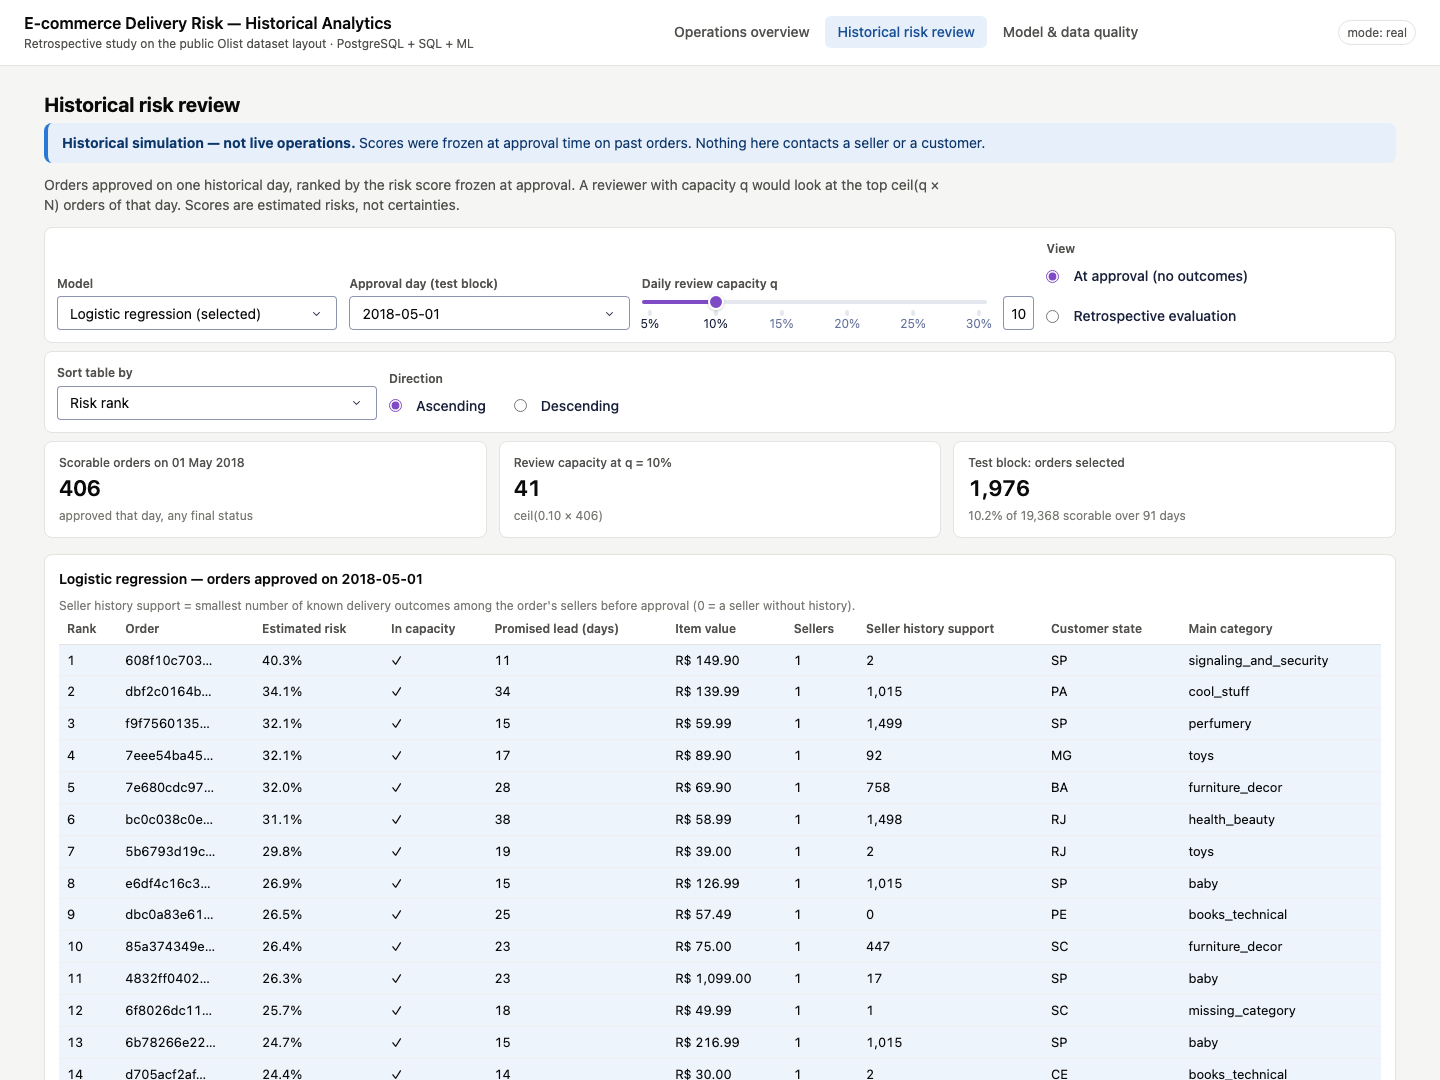
\includegraphics[width=0.9\linewidth]{figures/risk-review_1440_crop.png}
\caption{Historical risk review in \emph{At approval} mode: one approval day ranked by frozen score; the
capacity slider sets how many orders are flagged; no outcome is queried in this mode.}
\end{subfigure}
\caption{The application on the real data (screenshots at 1440\,px; the pages were also checked at
1024\,px).}
\label{fig:app}
\end{figure*}


Three representative queries were measured on the real volume in an isolated schema, with one warm-up
and five timed runs on \PGVersion{} (Docker, 8 vCPUs, 4\,GB). Each query was measured before and after
an index or a rewrite motivated by its \code{EXPLAIN (ANALYZE, BUFFERS)} plan, and the results were
checked to be identical (Table~\ref{tab:bench}).

\begin{table}[t]
\centering\scriptsize
\setlength{\tabcolsep}{2.5pt}
\caption{Server execution time (median of 5, ms) and index build time (ms). Q1: as-of history for
\NTargets{} targets against \NOutcomeEvents{} events; Q2: monthly overview aggregation; Q3: one day of
the risk review among \NPredictions{} stored scores.}
\label{tab:bench}
\begin{tabularx}{\columnwidth}{@{}l l X r r@{}}
\toprule
& Variant & Change & Time & Build \\
\midrule
\inputtable{generated/table_bench.tex}
\bottomrule
\end{tabularx}
\end{table}

\paragraph{Reading the plans.} For Q1, the \code{LATERAL} subquery runs once per distinct (seller, $t$).
Without an index each execution scans the whole event table, roughly $10^5$ targets times $10^5$
events, and the query was cancelled after \QOneBefore{}\,s. The composite index
\code{(seller\_id, outcome\_known\_at) INCLUDE (is\_late, ...)} turns that scan into an index-only range
scan of one seller's past (\QOneAfter{}\,s). A rewrite as a single event stream with
\code{RANGE BETWEEN INTERVAL '90 days' PRECEDING AND CURRENT ROW EXCLUDE GROUP}~\cite{pgdocs} needs no
index and returns the same rows, but takes \QOneWindow{}\,s here. With frame exclusion, PostgreSQL can
no longer maintain the window aggregate incrementally and re-aggregates every frame, which is costly
for sellers with long histories. Q3 changes from a sequential scan plus sort (\QThreeBefore{}\,ms) to an
index-only scan already in rank order (\QThreeAfter{}\,ms), so its index was kept. For Q2, a
sequential scan with a hash join already answers in \QTwoBefore{}\,ms; an index saved 5\,ms and was not
added. Query time is measured separately from rendering: the overview page takes \DashOverviewCold{}\,ms
to render with a cold cache and \DashOverviewWarm{}\,ms with a warm one.

% =====================================================================================
\section{The Application}\label{sec:app}

The Dash application reads the published tables through a read-only PostgreSQL role, in read-only
transactions, with bound parameters only. Sort columns come from an allow-list, page sizes are capped,
and results are cached under a key that includes the latest publication id, so a new pipeline run
invalidates the cache. It has three pages (Figure~\ref{fig:app}):
\begin{itemize}
\item \textbf{Operations overview.} Period, region and category filters; the date convention is
      displayed. Each KPI shows its denominator. Category filtering selects orders \emph{containing}
      a category, counted once. Segments and sellers below 30 eligible orders are hidden.
\item \textbf{Historical risk review.} One approval day of the test block ranked by frozen score, with a
      capacity slider. An \emph{At approval} mode never queries outcomes; a separate
      \emph{Retrospective evaluation} mode adds them with an explicit warning. A permanent banner
      states that this is a historical simulation, not live operations.
\item \textbf{Model \& data quality.} Model comparison with intervals, calibration, results by month
      and group (hidden below 30 orders or 10 late orders), split dates, data-quality checks and
      exclusions.
\end{itemize}
The application runs locally or in Docker (gunicorn). It is not deployed publicly. Doing so would
require a hosting choice, a reduced database dump containing only the published schemas, TLS to the
database, and a visible CC~BY-NC-SA attribution.


% =====================================================================================
\section{Limitations and Next Experiment}\label{sec:limits}

\begin{itemize}
\item \textbf{Snapshot data.} Promise, prices and catalog attributes could have changed after approval
      without trace. The ablation shows that the catalog assumption does not drive the results;
      the promise assumption cannot be tested in this source.
\item \textbf{Evaluated population.} Performance is measured on orders that were finally delivered.
      Scores of canceled or undelivered orders cannot be checked.
\item \textbf{Few weeks, strong seasonality.} With 14 test weeks the intervals are wide, performance
      depends heavily on the month's late rate, and calibration does not carry over between periods.
\item \textbf{Label cut-offs.} They are the right rule for an honest simulation, but here they left
      model selection with few late examples, and the choice it made was not the best on test.
\item \textbf{Shared outcomes.} Multi-seller orders share one delivery timestamp, and whether it refers
      to the first or the last parcel is not documented.
\item \textbf{No causal evidence.} A better-targeted queue is not proof that intervening helps.
\end{itemize}

\paragraph{Next experiment.} The question that matters, whether contacting the seller of a risky order
reduces lateness, requires an intervention. Each day, the top-$q$ orders would be split at random into
a \emph{contacted} and a \emph{not contacted} arm, so that both arms have the same score distribution.
Comparing late rates, delivery delays and review scores between the arms over several weeks measures
the effect of the action itself. The same pilot would collect the cost of each contact, which is needed
before any economic claim. The model would be recalibrated on recent deliveries before it starts.

% =====================================================================================
\section{Conclusion}

Most of the value of this project lies in what it refuses to count. Joins are checked against their
totals, so a silent \FanoutPct{} inflation cannot reach a dashboard. Features only see deliveries that
had happened, as an independent re-implementation confirms on every real row. The model is chosen
before the test block is opened, and the result is kept even when a rejected model turns out better. On
these terms, a simple logistic regression ranks risky orders measurably better than a seller-history
rule: AP \APSel{} vs \APRule{}, with a paired interval excluding zero. A 10\% daily review would have
worked on a queue \CapLift{} times richer in late orders. The gain is real but modest, and it depends on
the season. Turning it into a decision requires recalibration and the randomised pilot described above.

\small
\begin{thebibliography}{9}\setlength{\itemsep}{1pt}
\bibitem{olist} Olist, ``Brazilian E-Commerce Public Dataset by Olist,'' Kaggle, version 2, 2021. CC BY-NC-SA 4.0.
\bibitem{saito2015} T. Saito and M. Rehmsmeier, ``The Precision-Recall Plot Is More Informative than the ROC Plot When Evaluating Binary Classifiers on Imbalanced Datasets,'' \emph{PLoS ONE}, 10(3), 2015.
\bibitem{platt1999} J. Platt, ``Probabilistic Outputs for Support Vector Machines and Comparisons to Regularized Likelihood Methods,'' in \emph{Advances in Large Margin Classifiers}, MIT Press, 1999.
\bibitem{niculescu2005} A. Niculescu-Mizil and R. Caruana, ``Predicting Good Probabilities with Supervised Learning,'' \emph{Proc. ICML}, 2005.
\bibitem{lightgbm} G. Ke et al., ``LightGBM: A Highly Efficient Gradient Boosting Decision Tree,'' \emph{Advances in Neural Information Processing Systems}, 2017.
\bibitem{kunsch1989} H. R. K\"unsch, ``The Jackknife and the Bootstrap for General Stationary Observations,'' \emph{The Annals of Statistics}, 17(3), 1989.
\bibitem{kaufman2012} S. Kaufman, S. Rosset, C. Perlich and O. Stitelman, ``Leakage in Data Mining: Formulation, Detection, and Avoidance,'' \emph{ACM Transactions on Knowledge Discovery from Data}, 6(4), 2012.
\bibitem{sklearn} F. Pedregosa et al., ``Scikit-learn: Machine Learning in Python,'' \emph{Journal of Machine Learning Research}, 12, 2011.
\bibitem{pgdocs} PostgreSQL Global Development Group, \emph{PostgreSQL 17 Documentation}: ``Window Functions'' and ``Using EXPLAIN,'' 2024.
\end{thebibliography}

\end{document}
